\documentclass[11pt]{article}
\title{Meccano pentagons gallery}
\author{https://github.com/heptagons/meccano/penta/gallery}
\date{2023/12/3}

\usepackage{../../meccano}
\begin{document}

\maketitle
\begin{abstract}
We build rigid meccano regular pentagons from sides $12$ to $3$. We restrict all internal strips to remain inside the pentagon's perimeter and don't permit they overlap with others. We follow three steps. 1) We calculate distances between selected strips holes from the regular pentagons perimeter. 2) We run some programs available in this repo to look for rigid strips clusters which contains the distance. 3) We simplify or reduce the cluster to fit inside the pentagon. We prove the correctness of the cluster distance applied to check the software. We try each construction is relevant for the pentagon size.
\end{abstract}

\section{Pentagons of size 12}

A program found that side 12 is the smallest pentagon that can be made rigid with a rhoumbus and two strips as diagonals so need only 4 strips as diagonals. We show two cases.

\begin{figure}[h]
 \centering
 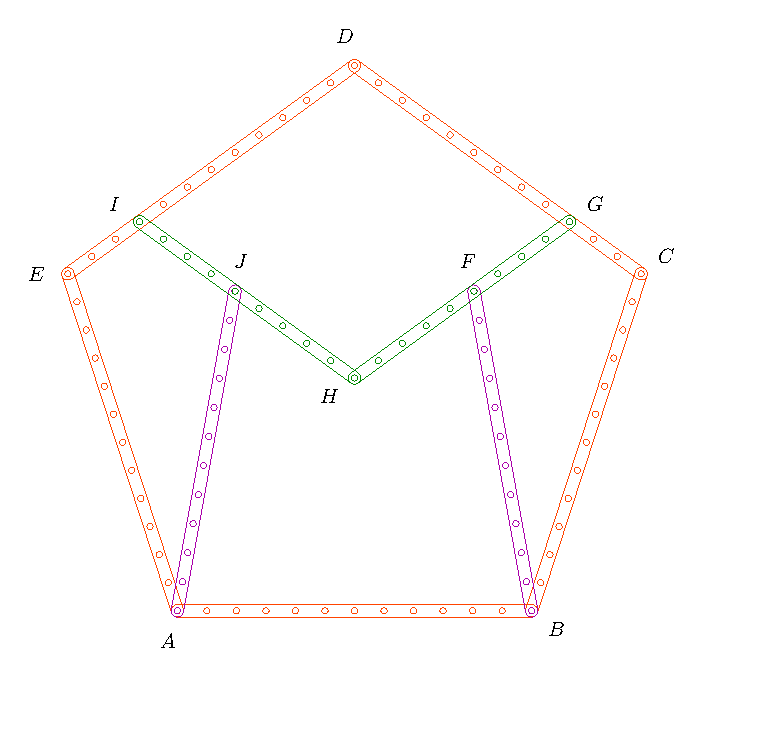
\includegraphics[scale=1]{12/penta12a}
 \caption{Regular pentagon size 12 (case a) made rigid with only four internal strips.}
 \label{fig:penta12a}
\end{figure}

Figure \ref{fig:penta12a} show a regular pentagon $A,B,C,D,E$ of side 12 with a rhombus $D,I,H,G$ of side $9$. We prove strips $AJ,BF$ are correct. First we calculate the abscissas going through vertices $A,E,I,J$ substracting when we move to the left and adding when we move to the right:
\begin{align}
AJ_x &= AE_x + EI_x + IJ_x\nonumber\\
 &= -\overline{AE}\cos\left(\frac{2\pi}5\right)
 + \overline{EI}\cos\left(\frac{\pi}5\right) 
 + \overline{IJ}\cos\left(\frac{\pi}5\right)\nonumber\\
 &= -12\left(\frac{\sqrt5 - 1}4\right)
  +3\left(\frac{1+\sqrt5}4\right)
  +4\left(\frac{1+\sqrt5}4\right) 
  = \frac{19-5\sqrt5}4
\end{align}

Then we calculate the ordinates going to the same order of vertices adding when we go up and substracting when we go down:
\begin{align}
AJ_y &= -AE_y + EI_y + IJ_y\nonumber\\
 &= \overline{AE}\sin\left(\frac{2\pi}5\right)
 + \overline{EI}\sin\left(\frac{\pi}5\right) 
 - \overline{IJ}\sin\left(\frac{\pi}5\right)\nonumber\\
 &= 12\left(\frac{\sqrt{10+2\sqrt5}}4\right)
 + 3\left(\frac{\sqrt{10-2\sqrt5}}4\right)
 - 4\left(\frac{\sqrt{10-2\sqrt5}}4\right)%\nonumber\\
 %&= \frac{12\sqrt{10+2\sqrt5} - \sqrt{10-2\sqrt5}}4 
 = \frac{\sqrt{1450+190\sqrt5}}4
\end{align}
Finally we calculate the distance $\overline{AJ}$ which coincides with strip size $11$:
\begin{align}
\overline{AJ} &= \sqrt{(AJ_x)^2 + (AJ_y)^2}\nonumber\\
 &= \sqrt{\left(\frac{19-5\sqrt5}4\right)^2 + \frac{1450+190\sqrt5}{16}}%\nonumber\\
 %&= \sqrt{\frac{486-190\sqrt5}{16} + \frac{1450+190\sqrt5}{16}} 
 = \sqrt{121} = 11
\end{align}

\begin{figure}[h]
 \centering
 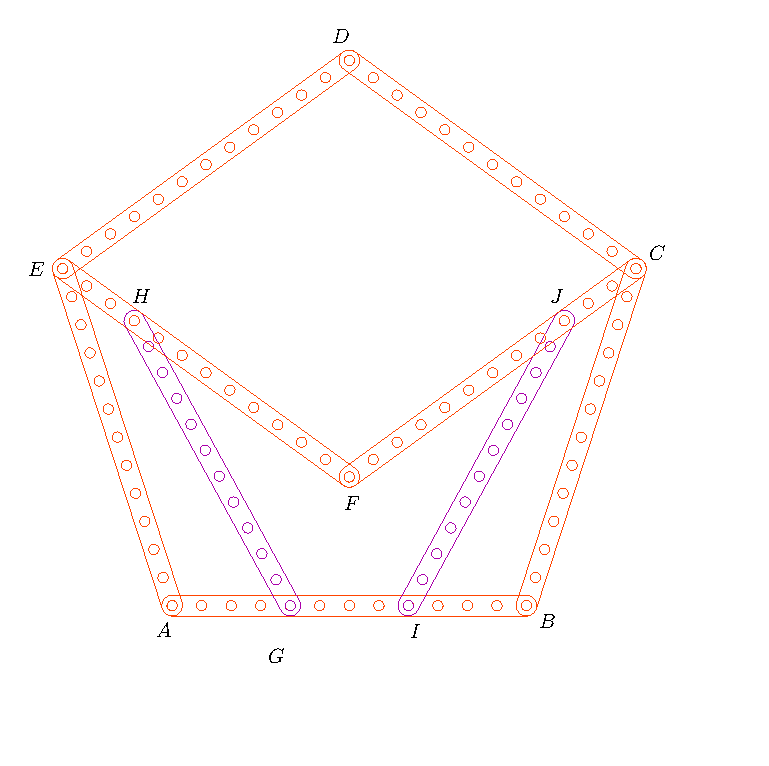
\includegraphics[scale=1]{12/penta12b}
 \caption{Regular pentagon size 12 case (b) made rigid with only four internal strips.}
 \label{fig:penta12b}
\end{figure}

Figure \ref{fig:penta12b} show a regular pentagon $A,B,C,D,E$ of size 12 with a rhombus $D,I,H,G$ of size $12$. We prove strips $GH,IJ$ are correct. First we calculate the abscissas going through vertices $G,A,E,H$ substracting when we move to the left and adding when we move to the right:
\begin{align}
GH_x &= -GA_x - AE_x + EH_x\nonumber\\
 &= -\overline{GA} - \overline{AE}\cos\left(\frac{2\pi}5\right)
 +\overline{EH}\cos\left(\frac{\pi}5\right)\nonumber\\
 &= -4 - 12\left(\frac{\sqrt5 - 1}4\right) + 3\left(\frac{1+\sqrt5}4\right)
 = \frac{-1-9\sqrt5}4
\end{align}

Then we calculate the ordinates going to the same order of vertices adding when we go up and substracting when we go down:
\begin{align}
GH_y &= AG_y + AE_y - EH_y\nonumber\\
 &= 0 + \overline{AE}\sin\left(\frac{2\pi}5\right)
 - \overline{EH}\sin\left(\frac{\pi}5\right)\nonumber\\
 &= 12\left(\frac{\sqrt{10+2\sqrt5}}4\right)
 - 3\left(\frac{\sqrt{10-2\sqrt5}}4\right)%\nonumber\\
 %&= \frac{12\sqrt{10+2\sqrt5} -3\sqrt{10-2\sqrt5}}4 
 = \frac{\sqrt{1530-18\sqrt5}}4
\end{align}

Finally we calculate the distance $\overline{GH}$ which coincides with strip size $11$:
\begin{align}
\overline{GH} &= \sqrt{(GH_x)^2 + (GH_y)^2}\nonumber\\
 &= \sqrt{\left(\frac{-1-9\sqrt5}{4}\right)^2 + \frac{1530-18\sqrt5}{16}}%\nonumber\\
 %&= \sqrt{\frac{406+18\sqrt5}{16} + \frac{1530-18\sqrt5}{16}} 
 = \sqrt{121} = 11
\end{align}


\section{Pentagon of size 11}

\begin{figure}[h]
 \centering
 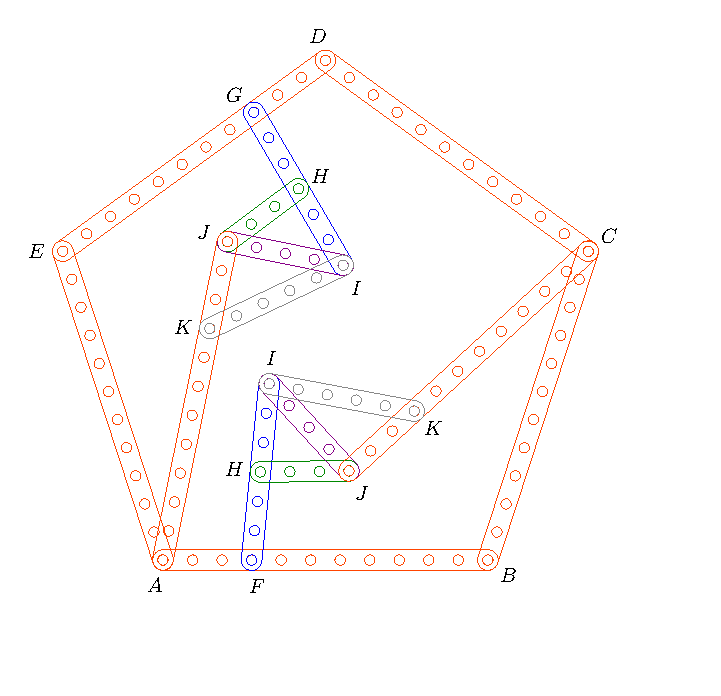
\includegraphics[scale=1]{11/penta11a}
 \caption{Regular pentagon size 11 made rigid with two internal clusters of five strips each.}
 \label{fig:penta11a}
\end{figure}

Figure \ref{fig:penta11a} show a rigid regular pentagon $A,B,C,D,E$ of size 11. A program found this is the smallest pentagon having a consecutive sides diagonal of the form $\dfrac{z_2 + z_3\sqrt5}{z_1}$ instead of the nested form $\dfrac{z_2\sqrt{z_3+z_4\sqrt5}}{z_1}$ where $z_i$ are integers. The mentioned diagonal is the distance $\overline{CF}$ in the figure which can be calculated with the law of cosines knowing angle $\angle{CBF} = \dfrac{3\pi}5$ and denesting the result. We calculate the angle $\angle{CFB}$ for the drawing:
\begin{align}
\overline{CF}^2 &= \overline{BC}^2 + \overline{BF}^2 
 - 2(\overline{BC})(\overline{BF})\cos\left(\dfrac{3\pi}5\right) \nonumber\\
 &= 11^2 + 8^2 - 2(11)(8)\left(\frac{1-\sqrt5}4\right) = 141 + 44\sqrt5 \nonumber\\
\overline{CF} &= \sqrt{141 + 44\sqrt5} = 11 + 2\sqrt5\\
%
\cos(\angle{CFB}) &= \frac{\overline{CF}^2 + \overline{BF}^2 - \overline{BC}^2}
 {2(\overline{CF})(\overline{BF})}%\nonumber\\
 = \frac{141+44\sqrt5 + 8^2 - 11^2}{2(11+2\sqrt5)(8)}
  = \frac{21+11\sqrt5}{44+8\sqrt5} = \frac{121+79\sqrt5}{404}
\end{align}

\subsection{Distance $11+2\sqrt{5}$}

A five strips cluster can create a rigid distance like $11 + 2\sqrt{5}$. In the figure, three strips $\overline{FI} = 2\overline{HJ}, \overline{FI} > \overline{IJ}$ builds a right angle $\angle{FJI} = \pi$, since triangle $\triangle{IJH}$ is isosceles ($\overline{FH} = \overline{HI} = \overline{JH}$). These three strips also build a distance $\overline{FJ} = \sqrt{\overline{FI}^2 - \overline{IJ}^2} = \sqrt{6^2 - 4^2} = 2\sqrt5$. Now we attach strip $\overline{CJ}$ making a second right triangle $\angle{CJI} = \pi$ using strip $\overline{IK}=5$ as pythagorean diagonal ($\overline{JK}=3, \overline{IJ}=4$). We have two right triangles at vertice $J$ so vertices $F,J,C$ are collinear, so we can calculate the distance $\overline{FC} = \overline{CJ} + \overline{JF} = 11 + 2\sqrt5$. We repeat the five-strips cluster between vertices $A,G$ preventing overlaps of any strips. Since the clusters are rigid we formed two rigid triangles $\triangle{ABC}, \triangle{DEA}$ so the pentagon is rigid.
\\\\
The program found the next pentagon of this type is a lot bigger: $\overline{BC}=246, \overline{BF}=70, \overline{CF}=41+105\sqrt5$.

\section{Pentagon of size 10}

\begin{figure}[h]
 \centering
 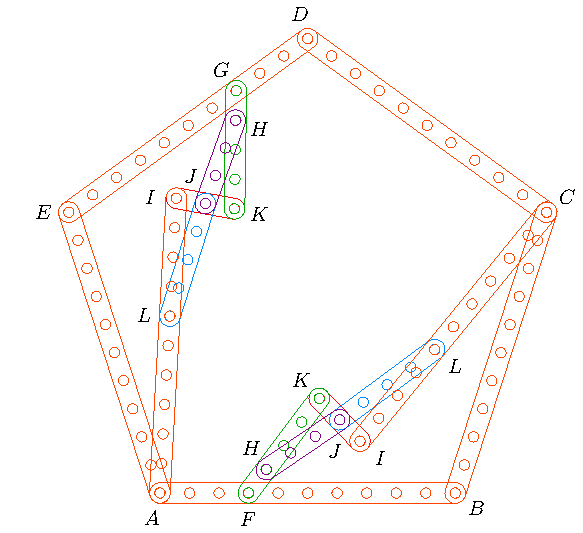
\includegraphics[scale=1]{10/penta10a}
 \caption{Regular pentagon size 10 made rigid with two internal clusters of five strips each.}
 \label{fig:penta10a}
\end{figure}

Figure \ref{fig:penta10a} show a rigid regular pentagon $A,B,C,D,E$ of size 10. We calculate a diagonal joining two consecutive sides relative primes to have something exclusive to the size 10, we choose $\overline{BF}:\overline{BC} = 7:10$. With the law of cosines we calculate $\overline{CF}$.
We calculate the angle $\angle{CFB}$ for the drawing:
\begin{align}
\overline{CF}^2 &= \overline{BC}^2 + \overline{BF}^2
 - 2(\overline{BC})(\overline{BF})\cos\left(\frac{3\pi}5\right) \nonumber\\
 &= 10^2 + 7^2 - 2(10)(7)\left(\frac{1-\sqrt5}4\right) = 114 + 35\sqrt5 \nonumber\\
\overline{CF} &= \sqrt{114 + 35\sqrt5} \\
\cos(\angle{CFB}) &= \frac{\overline{CF}^2 + \overline{BF}^2 - \overline{BC}^2}
 {2(\overline{CF})(\overline{BF})}%\nonumber\\
 = \frac{114+35\sqrt5 + 7^2 - 10^2}{2(\sqrt{114 + 35\sqrt5})(7)}
  = \frac{9+5\sqrt5}{2\sqrt{114+35\sqrt5}}
\end{align}

\subsection{Distance $\sqrt{114+35\sqrt5}$}

\begin{figure}[h]
 \centering
 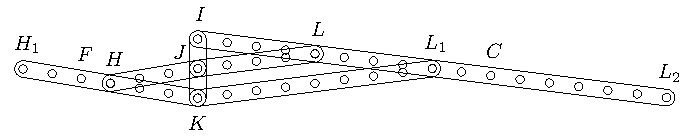
\includegraphics[scale=1.3]{10/cluster10a}
 \caption{Construction of distance $\overline{CF} = \sqrt{114+35\sqrt5}$}
 \label{fig:cluster10a}
\end{figure}

Number $\sqrt{114 + 35\sqrt5}$ cannot be denested so we need to solve this with a cluster of strips. A program found a lot of solutions for this distance using five strips, so we choose one narrow enough to fit inside the decagon.
\\\\
Figure \ref{fig:cluster10a} shows how to prove the cluster selected is correct. In the figure we have two isoscelles triangles $\triangle{IKL_1}$ and $\triangle{JKH}$. The sides $IL_1$ and $KH$ are extended to double the original size to the vertices $L_2$ and $H_1$ building two right angles $\angle{IKL_2}$ and $\angle{KJH_1}$. The right triangles permit the calculation of the abscissas and ordinates of vertices $C$ and $F$ to calculate their distance.
\\\\
From the figure we calculate $\overline{KL_2}$ and $\overline{JH_1}$ from their respective right triangles:
\begin{align}
\overline{KL_2} = \sqrt{(\overline{IL_2})^2 - (IK)^2} = \sqrt{16^2 - 2^2} = 6\sqrt7\\
\overline{JH_1} = \sqrt{(\overline{KH_1})^2 - (KJ)^2} = \sqrt{6^2 - 1^2} = \sqrt{35}
\end{align}

Assuming vertice $K$ is at the origin we can calculate the abscissas $C_x,F_x$ and ordinates $C_y,F_y$ of vertices $C$ and $F$ using as factors $c = \dfrac{\overline{IC}}{\overline{IL_2}} = \dfrac{10}{16} = \dfrac{5}8$ and $f = \dfrac{\overline{KF}}{\overline{KH1}}=\dfrac{4}6 = \dfrac{2}3$:
\begin{align}
C_x &= +c(\overline{KL_2}) = \frac{5}{8}(6\sqrt7) = \frac{15}{4}\sqrt7\\
F_x &= -f(\overline{JH_1}) = -\frac{2}{3}\sqrt{35}\\
C_y &= +(\overline{KI}) - c(\overline{KI}) = 2 - \frac{5}{8}(2) = \frac{3}4\\
F_y &= +f(\overline{KJ}) = \frac{2}{3}(1) = \frac{2}3
\end{align}

Finally we calculate the distance $\overline{CF}$:
\begin{align}
\overline{CF} &= \sqrt{(C_x - F_x)^2 + (C_y - F_y)^2}\nonumber\\
 &= \sqrt{\left(\frac{15}{4}\sqrt7 + \frac{2}{3}\sqrt{35}\right)^2
 + \left(\frac{3}4 - \frac{2}3\right)^2} %\nonumber\\
 %&= \sqrt{\dfrac{1575}{16} + 35\sqrt5 + \dfrac{140}9 + \dfrac{1}{144}} 
 = \sqrt{114+35\sqrt5}
\end{align}
A minimal part with five strips of the construction of figure \ref{fig:cluster10a} including only vertices $F,H,I,J,K,L,C$ is used twice to make rigid the pentagon of side 10 as show in figure \ref{fig:penta10a}.

\section{Pentagons of size 9}

\subsection{With 6 internal strips}

\begin{figure}[h]
 \centering
 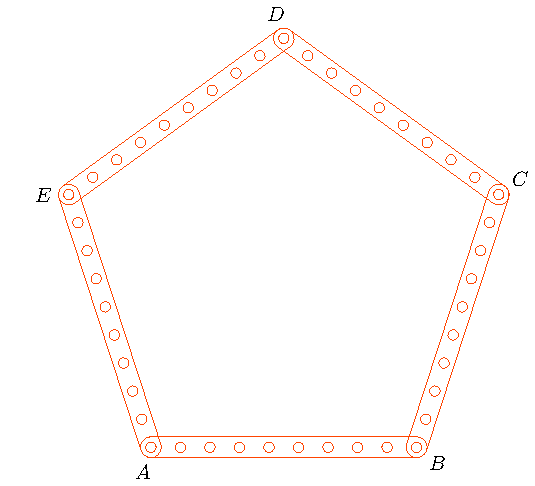
\includegraphics[scale=1]{9/penta9a}
 \caption{Regular pentagon size 9 (case a) made rigid with only six extra internal strips.}
 \label{fig:penta9a}
\end{figure}

Figure \ref{fig:penta9a} show a rigid regular pentagon $A,B,C,D,E$ of size $9$. The regular pentagon distance $\overline{CE}$ is called width and equals $\dfrac{1+\sqrt5}{2}\overline{AB}$. Is easy to note the distance $\overline{FG}$ equals the width of smaller pentagons size $9-1=8$ plus $1$. So we have:
\begin{align}
\overline{FG} &= \frac{1+\sqrt5}{2}(\overline{BC}-\overline{FC}) + \overline{FC}\nonumber\\
 &= \frac{1+\sqrt5}{2}(9-1) + 1 = 5 + 4\sqrt5
\end{align}

From the figure we see two right angles. Angle $\angle{GJK}=\pi$ because we have a Pythagorean triangle $\triangle{HJK}$. Angle $\angle{FJM}=\pi$ because we have an isosceles triangle $\triangle{FLM}$. The two right angles share vertice $J$ so vertices $G,J,F$ are collinear. First we calculate the distance $\overline{JF} = \sqrt{(LF)^2 - (LJ)^2} = \sqrt{9^2-1^2} = 4\sqrt5$ and finally the distance $\overline{GF} = \overline{GJ} + \overline{JF} = 5 + 4\sqrt5$ which matches the value in last equation above. To make rigid the pentagon we add strip $\overline{IN}$ parallel to side $\overline{GA}$.

\subsection{With 8 internal strips}

\begin{figure}[H]
 \centering
 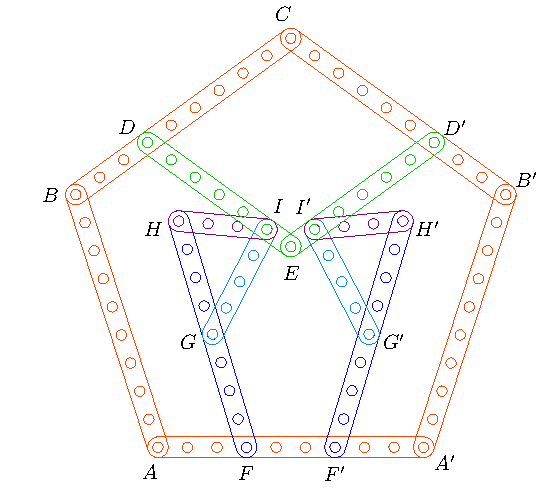
\includegraphics[scale=1]{9/penta9-8a}
 \caption{Regular pentagon size 9 made rigid with 8 strips variation I.}
 \label{fig:penta9-8a}
\end{figure}



\subsection{With 10 internal strips}

\begin{figure}[H]
 \centering
 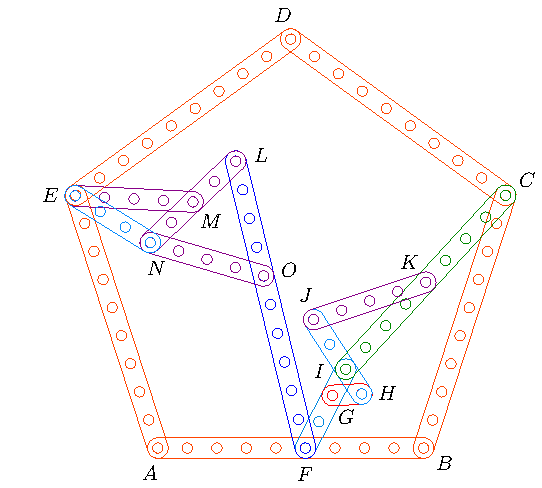
\includegraphics[scale=1]{9/penta9b}
 \caption{Regular pentagon size 9 (case b) made rigid with two internal clusters of five strips each.}
 \label{fig:penta9b}
\end{figure}

Figure \ref{fig:penta9b} show a regular pentagon $A,B,C,D,E$ of size $9$ made it rigid with the help of clusters fixing the distances $\overline{CF}$ and $\overline{EF}$. Pentagon size $9$ is the smaller one with diagonals where consecutive side segments fractions are $\overline{BF} / \overline{BC} =\dfrac{4}9$ and $\overline{AF} / \overline{AE} = \dfrac{5}9$. We calculate the diagonals $\overline{CF}$, $\overline{EF}$ and the angles to side $\overline{AB}$ using the law of cosines and the internal pentagon angle $\theta=\angle{FBC}=\angle{FAE}=\dfrac{3\pi}5$ where $\cos\theta = \dfrac{1-\sqrt5}4$:
\begin{align}
\overline{CF} &= \sqrt{
 \overline{BC}^2 + \overline{BF}^2 - 2(\overline{BC})(\overline{BF})\cos\theta } 
 = \sqrt{9^2 + 4^2 - 2(9)(4)\left(\frac{1-\sqrt5}4\right)} = \sqrt{79 + 18\sqrt5}\\
%
\cos(\angle{CFB}) &= 
 \frac{\overline{CF}^2 + \overline{BF}^2 - \overline{BC}^2}{2(\overline{CF})(\overline{BF})}
 = \frac{79 + 18\sqrt5 + 4^2 - 9^2}{2(\sqrt{79 + 18\sqrt5})(4)}
 = \frac{7 + 9\sqrt5}{4\sqrt{79 + 18\sqrt5}} \\
%
\overline{EF} &= \sqrt{
 \overline{AE}^2 + \overline{AF}^2 - 2(\overline{AE})(\overline{AF})\cos\theta} 
 = \sqrt{9^2 + 5^2 - 2(9)(5)\left(\frac{1-\sqrt5}4\right)} = \frac{\sqrt{334 + 90\sqrt5}}2\\
%
\cos(\angle{EFA}) &=
 \frac{\overline{EF}^2 + \overline{AF}^2 - \overline{EA}^2}{2(\overline{EF})(\overline{AF})}
 = \frac{\dfrac{334 + 90\sqrt5}4 + 5^2 - 9^2 }{2\left(\dfrac{\sqrt{334 + 90\sqrt5}}2\right)(5)}
 = \frac{11 + 9\sqrt5}{2\sqrt{334 + 90\sqrt5}}
\end{align}

Our software found several options with five strips to build distances $\sqrt{79 + 18\sqrt5}$
and $\dfrac{\sqrt{334 + 90\sqrt5}}2$.

\subsubsection{Distance $\sqrt{79 + 18\sqrt5}$}

\begin{figure}[H]
\centering
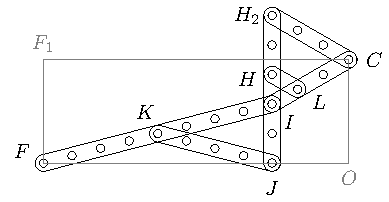
\includegraphics[scale=1]{9/cluster9b1}
\caption{Construction of distance $\overline{FC}=\sqrt{79 + 18\sqrt5}$}
\label{fig:cluster9b1}
\end{figure}

Figure \ref{fig:cluster9b1} show one of several ways to build the distance $\sqrt{79 + 18\sqrt5}$. 
Equilateral triangle $\triangle{FIZ}$ and isosceles $\triangle{IJK}$ share vertice $I$ and the base $\overline{JZ}$ which help to form rectangle $FXCY$ with base $\overline{FX}$ and height $\overline{FY}$ useful to calculate the diagonal $\overline{FC}$:
\begin{align}
\overline{FX} &= \overline{YJ} + \overline{JC}\nonumber\\
 &= \sqrt{\overline{FI}^2 - \left(\frac{\overline{IZ}}2\right)^2}
  + \sqrt{\overline{IC}^2 - \overline{IJ}^2}
  = \sqrt{3^2 - \left(\frac{3}2\right)^2} + \sqrt{8^2 - 2^2} 
  = \frac{3\sqrt3}2 + 2\sqrt{15} \nonumber\\
\overline{FY} &= \overline{JI} + \frac{\overline{IZ}}2
  = 2 + \frac{3}2 = \frac{7}2 \nonumber\\
\overline{FC} &= \sqrt{\overline{FX}^2 + \overline{FY}^2}
 = \sqrt{\left(\frac{3\sqrt3}2 + 2\sqrt{15}\right)^2 + \left(\frac{7}2\right)^2}
 = \sqrt{79 + 18\sqrt5}
\end{align}

We use a smaller part of this construction, the five strips with vertices $F,G,H,I,J,K,C$, as a cluster to made rigid the consecutive strips $\overline{AB},\overline{BC}$ of the pentagon of side $9$ of figure \ref{fig:penta9b}.


\subsubsection{Distance $\dfrac{\sqrt{334 + 90\sqrt5}}2$}

\begin{figure}[H]
\centering
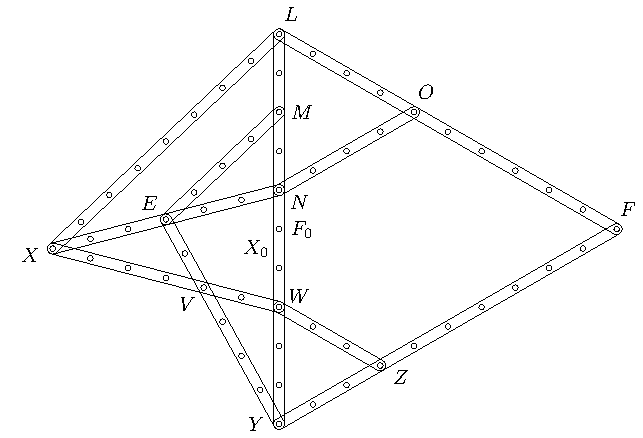
\includegraphics[scale=1]{9/cluster9b2}
\caption{Construction of distance $\overline{EF}=\dfrac{\sqrt{334 + 90\sqrt5}}2$}
\label{fig:cluster9b2}
\end{figure}

Figure \ref{fig:cluster9b2} show equilateral triangle $\triangle{FLY}$ and isoscelles triangle $\triangle{NXW}$ sharing strip $\overline{LY}$ which helps to calculate abscissas and ordinates of vertices $E,F$ to calculate distance $\overline{EF}$. Vertice $Y$ is located at the origin so:
\begin{align}
E_x &= - \left(\frac{\overline{NE}}{\overline{NX}}\right)\overline{XX_0}
 = -\frac{3}6\sqrt{\overline{NX}^2 - \overline{NX_0}^2}
 = -\frac{1}{2}\sqrt{6^2 - \left(\frac{3}2\right)^2} = -\frac{3\sqrt{15}}4 \\
E_y &= \overline{YN} - \left(\frac{\overline{NE}}{\overline{NX}}\right)\overline{NX_0}
 = 6 - \left(\frac{3}6\right)\left(\frac{3}2\right) = \frac{21}4\\
F_x &= \overline{F_0F} = \sqrt{\overline{YF}^2 - \overline{YF_0}^2}
 = \sqrt{10^2 - 5^2} = 5\sqrt3\\
F_y &= \overline{YF_0} = 5\\
\overline{EF} &= \sqrt{(E_x - F_x)^2 + (E_y - F_y)^2}
 = \sqrt{\left(-\frac{3\sqrt{15}}{4} -5\sqrt3 \right)^2 + \left(\frac{21}4 - 5\right)^2}
 = \frac{\sqrt{334+90\sqrt5}}2
\end{align}
We form a cluster from the last construction to be applied in the pentagon of side $9$. We choose the five strips with vertices $E,N,M,L,O,F$. Is easy to prove strip $\overline{EM}$ is correct in the cluster comparing equal cosines at vertice $Y$ for triangles $\triangle{YVW},\triangle{YEN},\triangle{YEM}$ using the law of cosines for each triangle.

\section{Pentagons of size 8}


\end{document}